\subsection{Preissmann scheme}\label{subse:preissmann_scheme}
From section \ref{se:hydraulics_of_sewer_line} the equations for an open channel is derived. In this section these Saint Venant equations are solved using a numerical method. 

%Argument for at bruge numeriske metode til at løse saint venant eq.

The numerical method used for solving the Saint Venant equations described in \ref{se:hydraulics_of_sewer_line} is the Preissmann scheme also known as the box scheme. Other method exist such as, Lax scheme, Abbot-Ionescu scheme, leap-frog scheme, Vasiliev scheme, however the Preissmann scheme is commonly known as the most robust scheme. By using the Preissmann scheme the Saint Venant equations can be discretized, and thereby used in a simulation to calculate the flow and height throughout an open channel.   

From section \ref{se:hydraulics_of_sewer_line} the Saint Venant equations for conductivity and momentum are derived, they are also shown below,

\begin{equation}\label{eq:saintbernard_mass_preiss}
\frac{\partial A(x,t)}{\partial t} + \frac{\partial Q(x,t)}{\partial x}=q(x,t)
\end{equation}

\begin{equation}\label{eq:saintbernard_momentum_preiss}
	\frac{\partial Q(x,t)}{\partial t} + \frac{\partial}{\partial x} \frac{Q^2(x,t)}{A(x,t)}+ g A(x,t) (\frac{\partial Y(x,t)}{\partial x} +S_f(x,t)-S_b(x)) = 0
\end{equation}

%Skriv noget om boundary og initial conditions

In figure \ref{fig:preissmann_grid_scheme} a single mesh is illustrated.

\begin{figure}[H]
\centering
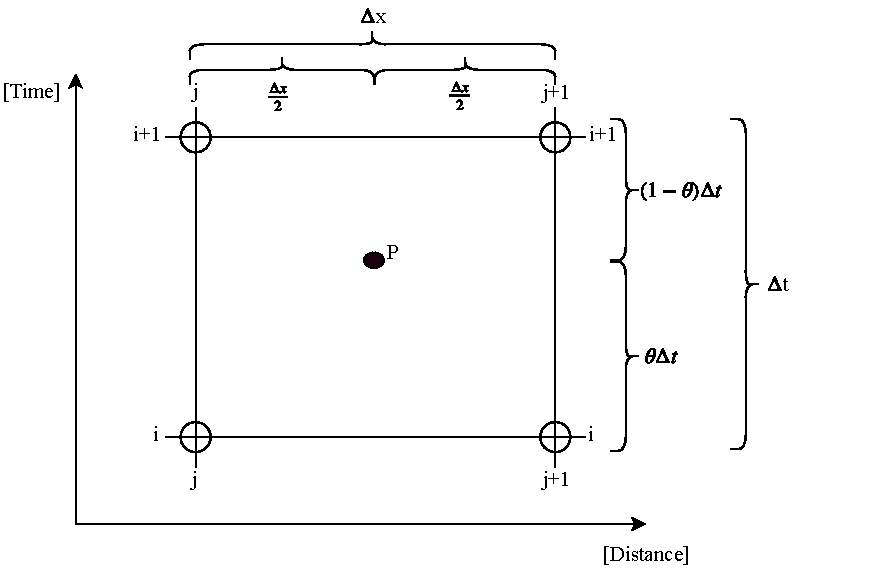
\includegraphics[width=.6\textwidth]{report/modeling/pictures/preissmann_scheme}
\caption{Preissmann non-staggered grid scheme.}
\label{fig:preissmann_grid_scheme}
\end{figure} 

Where $\theta$ is a weighting parameter ranging between 0 and 1, j index of section and i index of time. This mesh contains four nodes, (j,i), (j+1,i), (j,i+1) and (j+1,i+1), however in the implementation the dimension of the grid is $\Delta t \times \Delta x$ for $0 \leq x \leq L$ and $0\leq t$. Where L defines the length of the open channel. The derivatives in equations \ref{eq:saintbernard_mass_preiss} and \ref{eq:saintbernard_momentum_preiss} are calculated as approximation at the point P, which is in the middle of the interval $\Delta x$. Therefore the Preissmann scheme corresponds to a box scheme with a $\phi =0,5$. The point P can move along the t axis within this mesh by adjusting the weighting parameter $\theta$. This weighting parameter will be elaborated on later. An arbitrary function $f_p(x,t)$ calculated at point P is approximated by, 

\begin{equation}\label{eq:approximated_function}
	f_p \approx \frac{1}{2} (\theta \cdot f_j^{i+1}+(1-\theta)f_j^i)+\frac{1}{2}(\theta\cdot f_{j+1}^{i+1}+(1-\theta)f_{j+1}^i)
\end{equation}
The numerical approximation for the derivatives in equations \ref{eq:saintbernard_mass_preiss} and \ref{eq:saintbernard_momentum_preiss} for time and space are shown below, 

\begin{equation}\label{eq:preissmann_time_derivatie}
	\frac{\partial f}{\partial t}\bigg \rvert_p \approx \frac{1}{2}\left(\frac{f_j^{i+1}-f_j^n}{\Delta t}+\frac{f_{j+1}^{i+1}-f_{j+1}^i}{\Delta t}\right)
\end{equation}

\begin{equation}\label{eq:preissmann_space_derivatie}
	\frac{\partial f}{\partial x}\bigg \rvert_p \approx (1-\theta)\frac{f_j^i-f_{j+1}^i}{\Delta x}+\theta \frac{f_j^{i+1}-f_{j+1}^{i+1}}{\Delta x}
\end{equation}

These approximations from equations \ref{eq:preissmann_time_derivatie} and \ref{eq:preissmann_space_derivatie} can therefore inserted for the derivatives in the Saint Venant equations \ref{eq:saintbernard_mass_preiss} and \ref{eq:saintbernard_momentum_preiss} and thereby achieve the following, 

\begin{equation}\label{eq:continuity_eq_preissmann}
	\theta \frac{Q_{j+1}^{i+1}-Q_j^{i+1}}{\Delta x}+(1-\theta)\frac{Q_{j+1}^i - Q_j^i}{\Delta x}+
	\frac{A_{j+1}^{i+1}-A_{j+1}^i}{\Delta t}+\frac{A_{j}^{i+1} - A_j^i}{\Delta t} = q_p
\end{equation}

\begin{multline}
	\frac{1}{2} \left(\frac{Q_{j+1}^{i+1}-Q_{j+1}^i}{\Delta t}+\frac{Q_{j}^{i+1} - Q_j^i}{\Delta t}\right) + \frac{\theta}{\Delta x} \left(\left(\frac{Q^2}{A}\right)_{j+1}^{i+1}-\left(\frac{Q^2}{A}\right)_{j}^{i+1}\right) + \\ \frac{1-\theta}{\Delta x}\left(\left(\frac{Q^2}{A}\right)_{j+1}^{i}-\left(\frac{Q^2}{A}\right)_{j}^{i}\right)+gA_p\theta \left(\frac{h_{j+1}^{i+1}-h_j^{i+1}}{\Delta x}\right)+ \\ gA_p(1-\theta)\left(\frac{h_{j+1}^{i} - h_j^i}{\Delta x}\right)+\left(\frac{g\cdot n_M^2}{R^\frac{4}{3}}\frac{|Q|Q}{A}\right)_P = 0 
\end{multline}

By discretized the Saint Venant equations they can be used in a simulation to calculate parameters for the open channel model. The mesh shown in figure \ref{fig:preissmann_grid_scheme} is used to calculate the node (j+1,i+1) by knowing the previous values in time and space (j,i), (j+1,i) and (j,i+1). Some initial condition must be known to calculate the parameters for the open channel. The flow must be known throughout the pipe for time equal to zero, furthermore the flow that will enter the channel for $t\leq 0$ must be known, as shown in figure \ref{fig:preissmann_grid_scheme_exampel}.   

\begin{figure}[H]
\centering
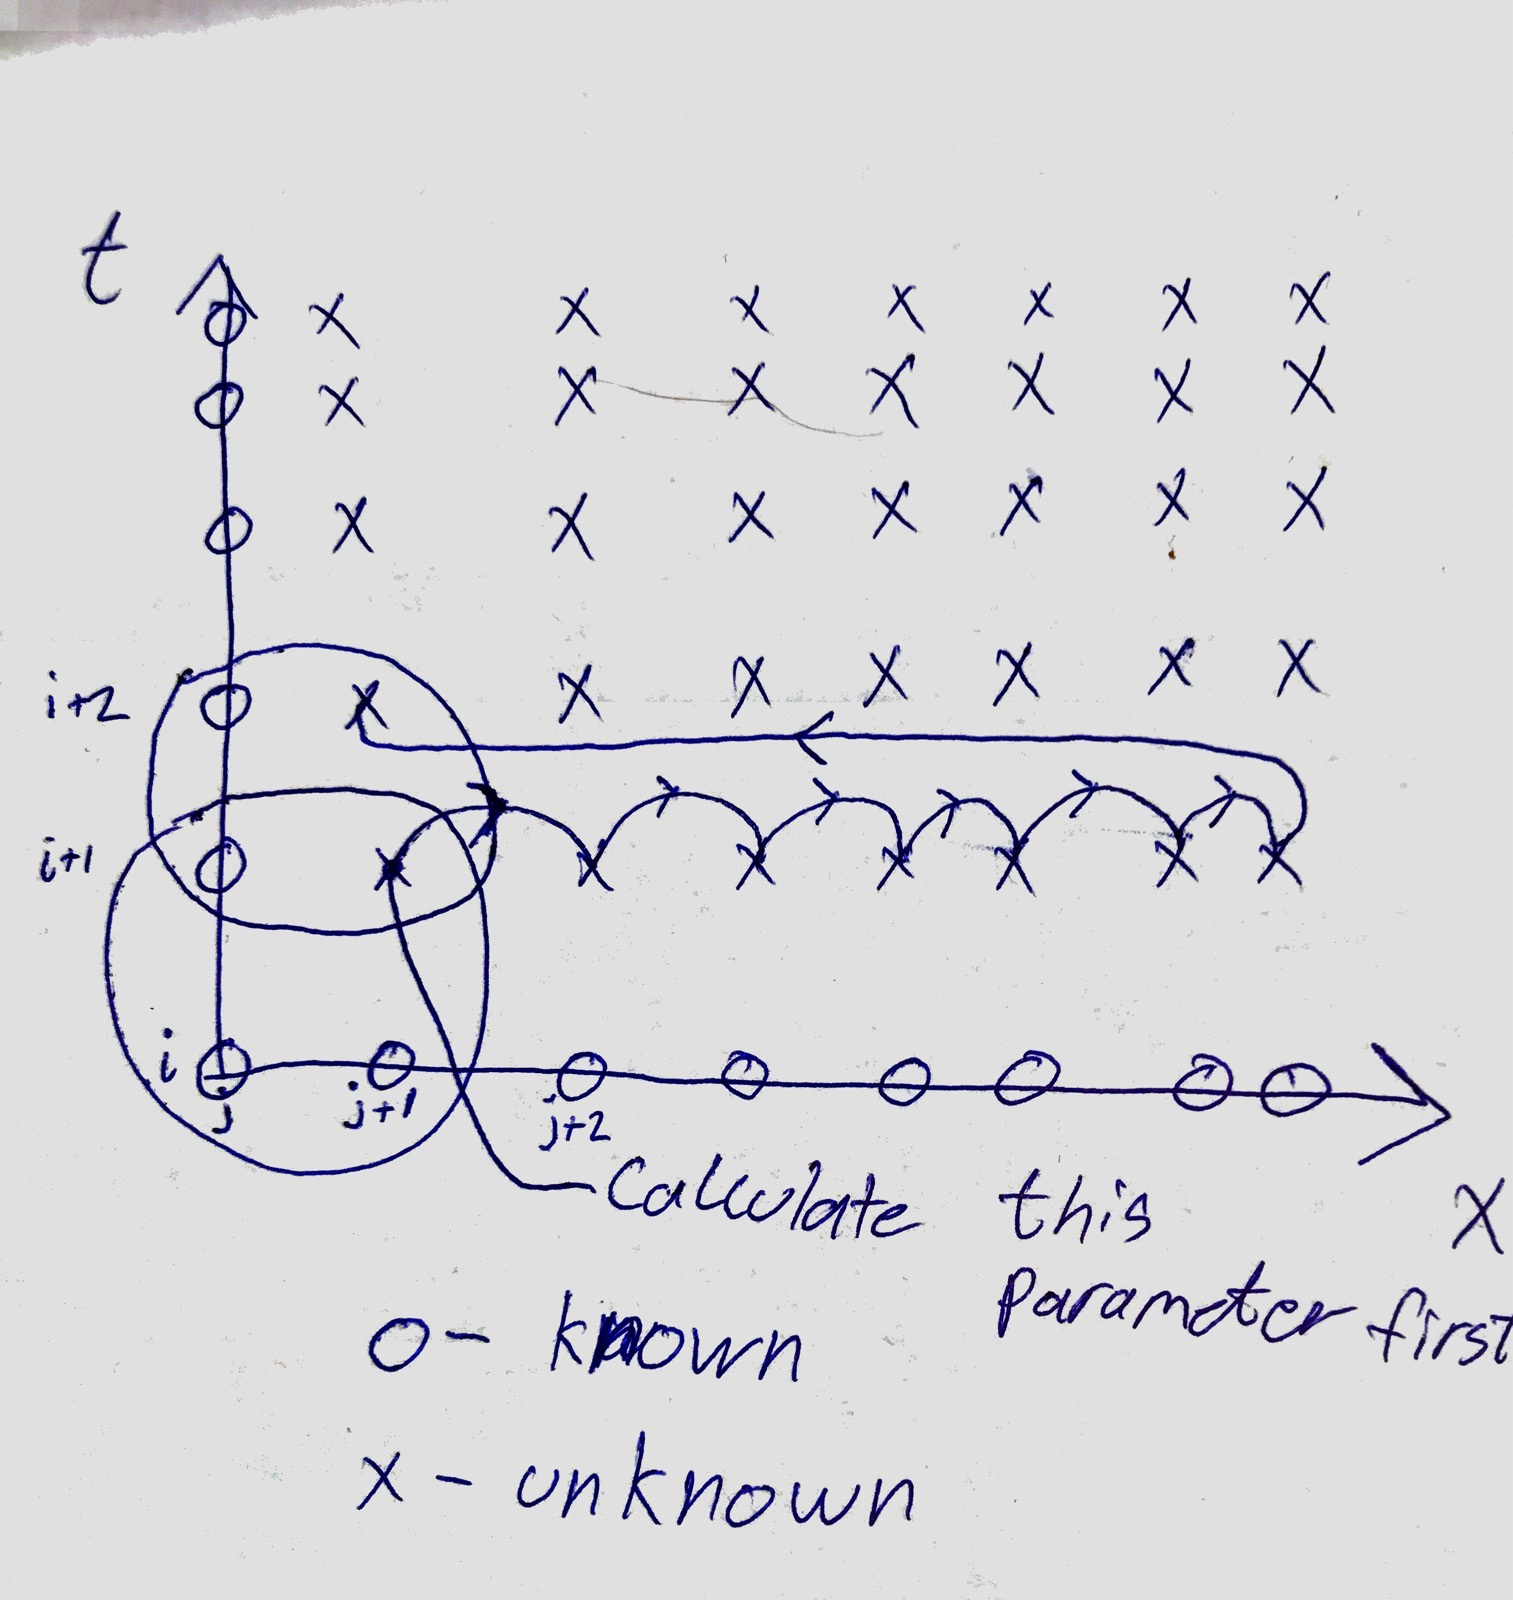
\includegraphics[width=.6\textwidth]{report/modeling/pictures/preissmann_scheme_exempel}
\caption{Preissmann non-staggered grid scheme example of calculation pattern.}
\label{fig:preissmann_grid_scheme_exampel}
\end{figure} 

By knowing the flow, and parameters for the pipe, the height can be calculated in the initialization nodes. With equation \ref{eq:continuity_eq_preissmann}, the flow and the height in (j,i), (j+1,i) and (j,i+1) by knowing these the flow and height can be computed for (j+1,i+1) with the help of equation \ref{eq:continuity_eq_preissmann} and the newton method, which will be elaborated on later.  

For the Preissmann scheme to be numerical stable the $\theta$ parameter is $\theta \leq 0,5$. If $\theta$ is equal to 0,5 the Preissmann scheme is second order accurate in both time and space, and is first order accurate otherwise.   

In the following section the calculating of the flow and height in each node will be explained.

\subsubsection*{Continuity equation}
In this section the scheme for calculating the flow and height in each iteration will be explained. 

The discretized continuity equation \ref{eq:continuity_eq_preissmann} from section \ref{subse:preissmann_scheme} is solved for the desired flow,

\begin{equation}
	Q_{j+1}^{i+1} = - \frac{1}{2\theta}\left(A_{j+1}^{i+1}-H\right)\frac{\Delta x}{\Delta t}
\end{equation}

Where H is a parameter where all the previous flows and areas are known,
\begin{equation}
	H = \left(2(1-\theta)Q_j^i-2(1-\theta)Q_{j+1}^i+2\theta Q_j^{i+1}+2q(x,t)\Delta x\right)\frac{\Delta t}{\Delta x}- A_{j}^{i+1}+A_j^i+A_{j+1}^i
\end{equation}

Where q is the inlet flow across a channel,
\begin{equation}
	q(x,t) = 0.25(q_j^i+q_j^{i+1}+q_{j+1}^{i+1}+q_j^{i+1})	
\end{equation}



\begin{equation}
		0=-Q_{j+1}^{i+1}  - \frac{1}{2\theta}\left(A_{j+1}^{i+1}-H\right)\frac{\Delta x}{\Delta t}
\end{equation}

\begin{equation}
		V=-Q_{j+1}^{i+1}  - \frac{1}{2\theta}\left(A_{j+1}^{i+1}-H\right)\frac{\Delta x}{\Delta t}
\end{equation}

\begin{equation}
	V = -Q_f\left(0,46-0,5cos\left(\pi \frac{h_{j+1}^{i+1}}{d}\right)+0,04cos\left(2\pi\frac{h_{j+1}^{i+1}}{d}\right)\right)\frac{\Delta t}{\Delta x}-\frac{1}{2\theta}\left(A_{j+1}^{i+1}-H\right)
\end{equation}

\begin{equation}
	V = -72\left(\frac{d}{4}\right)^{0.635}\pi\left(\frac{d}{2}\right)^2I_e^{0,5}\left(0,46-0,5cos\left(\pi \frac{h_{j+1}^{i+1}}{d}\right)+0,04cos\left(2\pi\frac{h_{j+1}^{i+1}}{d}\right)\right)\frac{\Delta t}{\Delta x}-\frac{1}{2\theta}\left(A_{j+1}^{i+1}-H\right)
\end{equation}

